\documentclass{beamer}
\usepackage{amsthm}
\usepackage{amssymb}
\usepackage{amsmath}
\usepackage{amsfonts}
\usepackage{graphicx}
\usepackage{tikz}
\usetheme{Rochester}
\usecolortheme{seahorse}
\usefonttheme{structuresmallcapsserif}
\setbeamertemplate{caption}[numbered]
\setbeamertemplate{footline}[frame number]
\usepackage{subfigure}


\title{Efficient segmentation algorithms for shark fin identification}
\subtitle{Honours project proposal}
\author{Lize Cilli\'{e}, Project advisors: Dr. S.J. van der Walt and Prof. B.M. Herbst}
\date{1 August 2013}
\institute{Department of Applied Mathematics, Stellenbosch University}

\begin{document}
\maketitle


\begin{frame}
\frametitle{Motivation and problem statement}
\begin{itemize}
\item Sharks have an unique dorsal fin structure.
\item The value of analysing shark fins.
\item Motivation behind the project.
\begin{itemize}
 \item 
 \item
\end{itemize}
\item Methodology.
\begin{itemize}
 \item 
 \item
\end{itemize}
\item Advantage for biological researchers.
\begin{itemize}
 \item
\end{itemize}
\item Examples of shark fins.
\end{itemize}
\end{frame}


\begin{frame}
\frametitle{Examples of shark fin images showing the unique dorsal part}
\begin{figure}
\centering
\mbox{\subfigure[Shark fin 1]{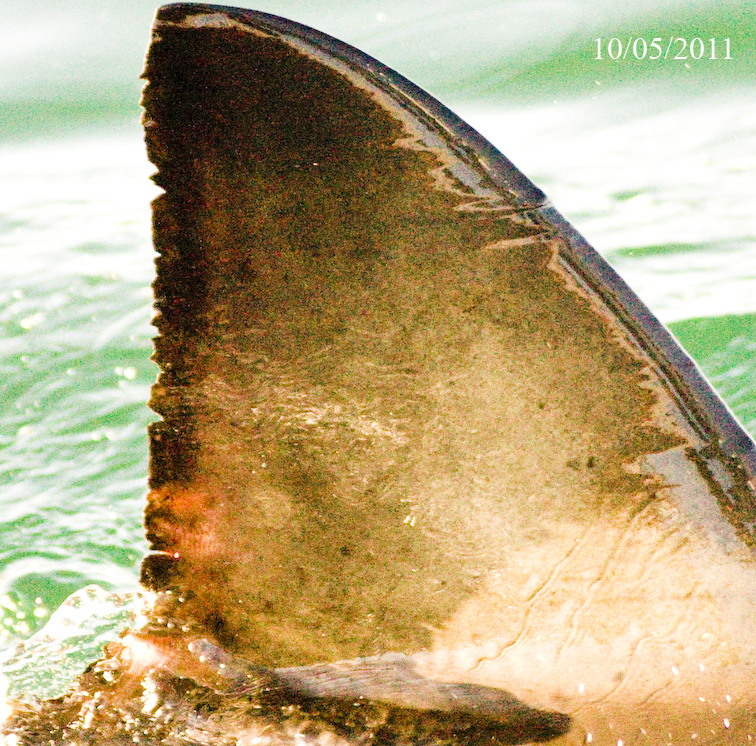
\includegraphics[width=1in]{haai1.jpg}} \quad
\subfigure[Shark fin 2]{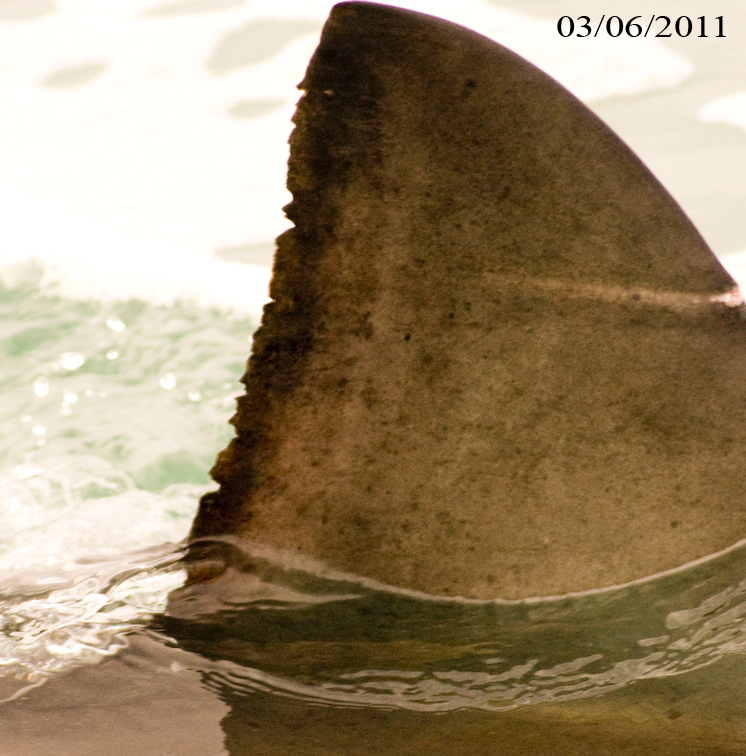
\includegraphics[width=1in]{haai2.jpg}}}
\end{figure}
\begin{figure}
\centering
\mbox{\subfigure[Shark fin 3]{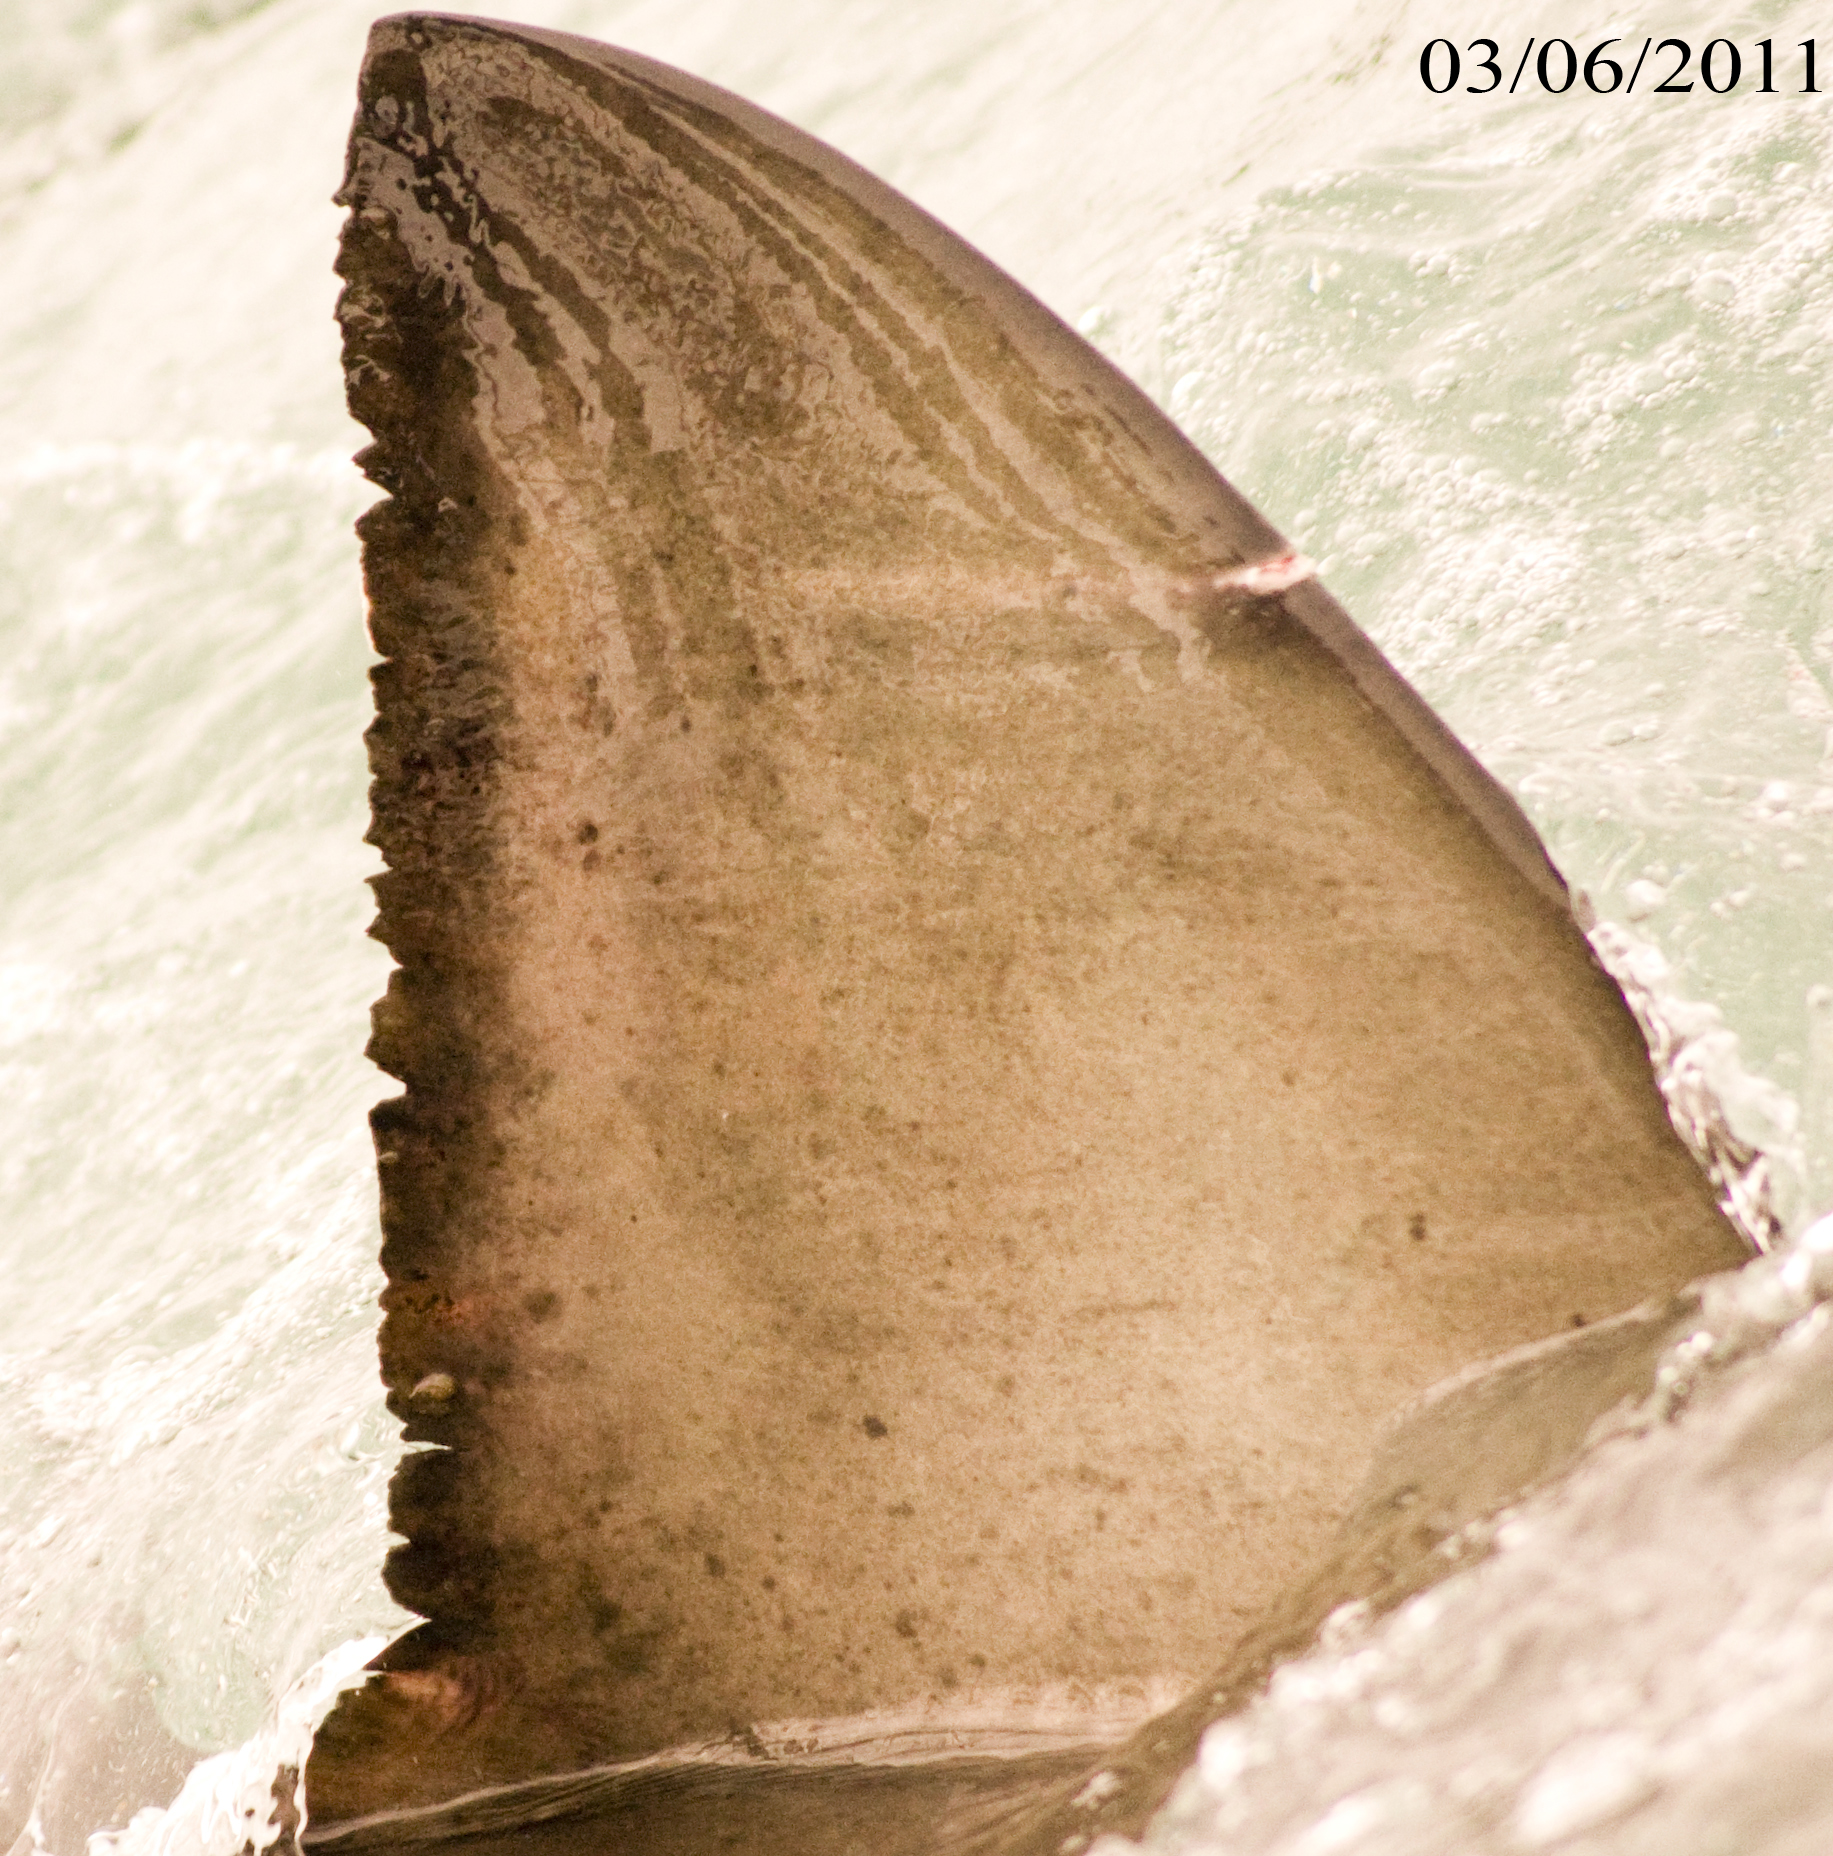
\includegraphics[width=1in]{haai3.jpg}} \quad
\subfigure[Shark fin 4]{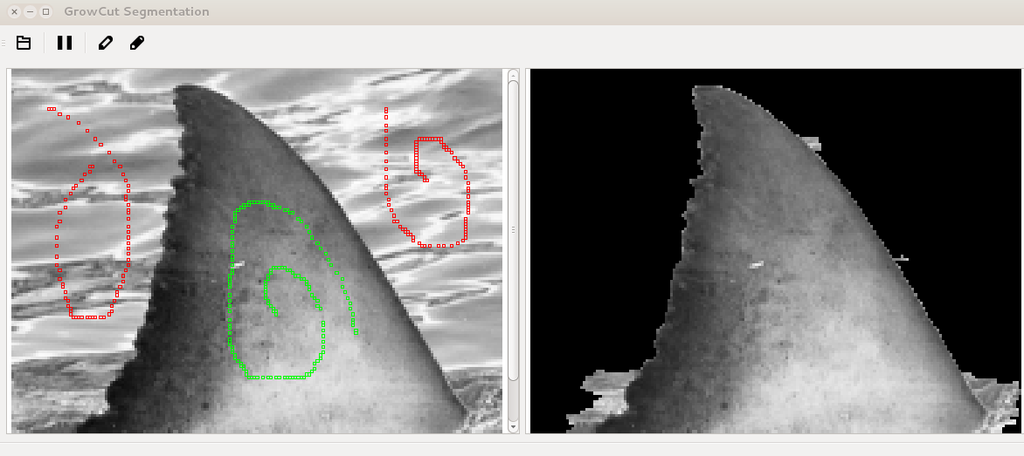
\includegraphics[width=1in]{haaim.png}}}
\end{figure}
\end{frame}


\begin{frame}
\frametitle{Background}
\begin{itemize}
\item Basic principle of segmentation algorithms.
\begin{itemize}
\item Partitioning a digital image into multiple segments to locate an object or boundaries in the image.
\end{itemize}
\item Applications.
\begin{itemize}
\item Medical imaging to locate tumours.
\begin{figure}
 \centering
 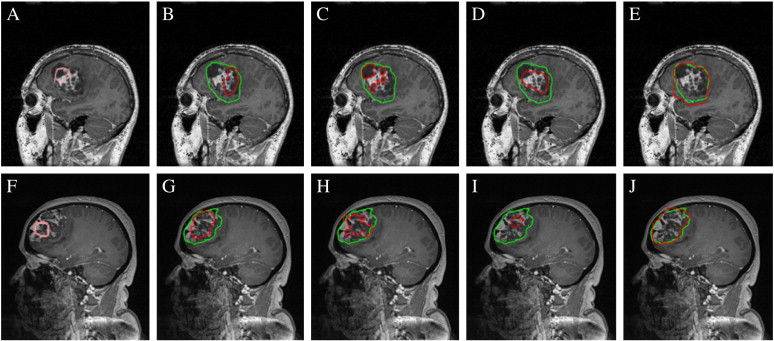
\includegraphics[width=2in]{braintumor.jpg}
 \caption{}
 \end{figure}
\item Face and fingerprint recognition.
\item Video surveillance.
\end{itemize}
\item Many different techniques.
\end{itemize}
\end{frame}

\begin{frame}
\frametitle{Algorithms from the scikit-image Python library}
\begin{itemize}
\item The Watershed\cite{scikit-image} algorithm.
\begin{itemize}
\item Method?
\item Challenge?
\end{itemize}
\begin{figure}
 \centering
 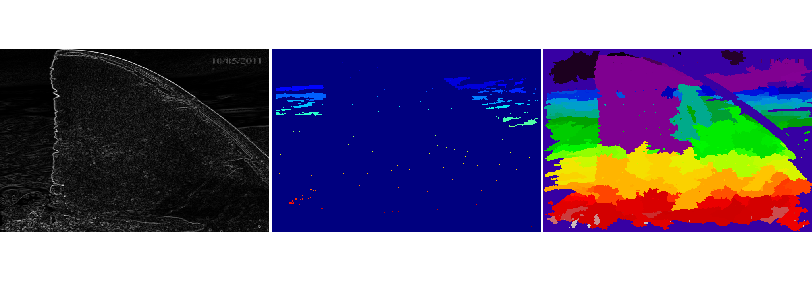
\includegraphics[width=2in]{watershed.png}
 \caption{}
 \end{figure}

\item The Random Walker\cite{scikit-image} algorithm.
\begin{itemize}
\item Method?
\item Challenge?
\end{itemize}
\end{itemize}
\end{frame}

\begin{frame}
\frametitle{The region growing Grow Cut segmentation algorithm}
\begin{itemize}
\item How does it work?
\begin{itemize}
\item Cellular Automata\cite{cellularoutomata}.
\item
\item
\item Attacking strategies/evolution rule.
\end{itemize}
\begin{figure}
\centering
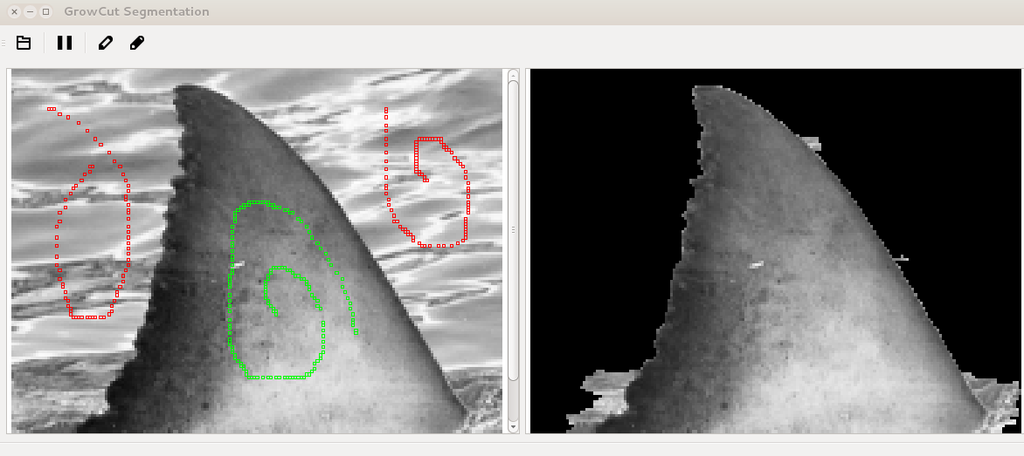
\includegraphics[width=1.5in]{haaim.png}
\caption{}
\end{figure}
\item Dr. Nathan Faggian\cite{NathanFaggian}.
\item Python implementation and Cython.
\item 
\end{itemize}
\end{frame}


\begin{frame}
\frametitle{DARWIN -- Alternative software}
\begin{itemize}
\item DARWIN\cite{Darwin} is open source software, allowing marine scientists to maintain information for the study of various behavioural and ecological patterns of bottlenose dolphins.
\item The software also makes use of images of the dorsal fin of the dolphin, on which segmentation then takes place.
\end{itemize}
\begin{figure}
 \centering
 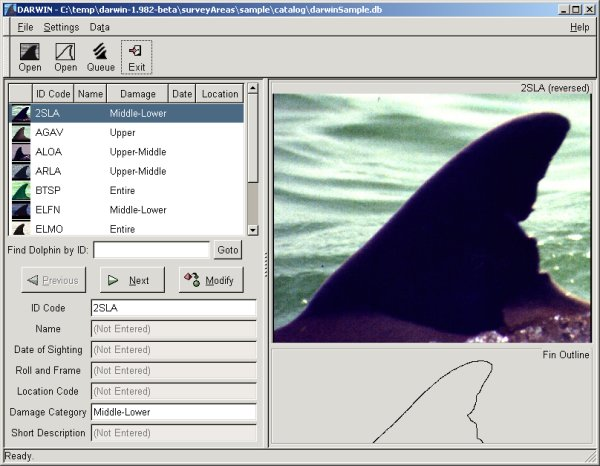
\includegraphics[width=1.5in]{Darwin.jpg}
 \caption{User interface}
\end{figure}
\end{frame}

\begin{frame}
\begin{itemize}
\item An article\cite{DieBurger} appeared in Die Burger claiming that this software could also be used to estimate the size of the Great White shark population in the Gansbaai area by means of shark fin identification and matching.
\item The validity of this claim was tested by Ms. Andreotti, which found it to be unreliable in 54\% of the cases.
\item Motivation.
\end{itemize}
\end{frame}


\begin{frame}
\frametitle{Work in progress} 
\begin{itemize}
\item We found that the Grow Cut algorithm performed the best on our data and focused our attention on that.
\item Putting together a pipeline for Ms. Andreotti, in collaboration with Tessa Marais, a MsC student in Applied Mathematics, Stellenbosch University.
\item Current challenges and solutions.
\begin{itemize}
\item Specification of the coordinates and setting the orientation.
\end{itemize}
\item Future work.
\begin{itemize}
\item
\end{itemize}
\end{itemize}
\end{frame}


\begin{frame}
\frametitle{Conclusions}
\begin{itemize}
\item Satisfaction of a project of this degree.
\item Demo of the Grow Cut algorithm.
\end{itemize}
\end{frame}


\begin{frame}
\frametitle{Bibliography}
\bibliographystyle{plain}
\bibliography{ProjectProposalPresentation}
\end{frame}


\end{document}
